% This is a Homework Template for CS 1010.  
% It was modified by  Michael Carl Tschantz (mtschant) 
% who provided the ``useful infomation on latex''.

% THE ONLY THING YOU NEED TO DO IN THIS PART IS 
% TO FILL IN THE HOMEWORK NUMBER, YOUR NAME AND LOG IN BELOW
% REPLACE ``X'' WITH THE HW NUMBER, ``Your Name'' WITH YOUR NAME,
% AND ``your login'' WITH YOUR LOGIN.

\newcommand{\hwnumber}{12}
\newcommand{\yourname}{Michael Mueller}

% NOW YOU MAY SKIP DOWN TO THE PART CALLED ``YOUR DOCUMENT''.

%==============================================================================
% Formatting parameters (how the page is set up)
%==============================================================================
\newcommand{\yourcourse}{Math 695}
\newcommand{\chapter}{0}
\newcommand{\mgn}{\mathcal M_{g,n}}
\newcommand{\mgnb}{\overline{\mathcal M_{g,n}}}
\newcommand{\mgb}[1]{\overline{\mathcal M_{g,#1}}}

\documentclass[11pt]{article}           % 11pt article
\makeatletter                   % Make '@' accessible.
\pagestyle{myheadings}              % We do our own page headers.
\newcommand{\thishw}{\bf Thesis}
\def\@oddhead{\bf \thishw \hfill \yourname}
\oddsidemargin=0in              % Left margin minus 1 inch.
\evensidemargin=0in             % Same for even-numbered pages.
\textwidth=6.5in                % Text width (8.5in - margins).
\topmargin=0in                  % Top margin minus 1 inch.
\headsep=0.2in                  % Distance from header to body.
\textheight=8in                 % Body height (incl. footnotes)
\skip\footins=4ex               % Space above first footnote.
\hbadness=10000                 % No "underfull hbox" messages.
\makeatother                    % Make '@' special again.

%==============================================================================
% Packages used (packages add more commands)
%==============================================================================

\usepackage{amsmath}                % give more fonts and symbols
\usepackage{amsfonts}               % want AMS fonts
\usepackage{amssymb}
\usepackage{amsthm}
\usepackage{mathrsfs}
\usepackage{tikz-cd}
\usepackage[shortlabels]{enumitem}
\usepackage{relsize}
\usepackage{hyperref}

\makeatletter
\newcommand*{\relrelbarsep}{.386ex}
\newcommand*{\relrelbar}{%
  \mathrel{%
    \mathpalette\@relrelbar\relrelbarsep
  }%
}
\newcommand*{\@relrelbar}[2]{%
  \raise#2\hbox to 0pt{$\m@th#1\relbar$\hss}%
  \lower#2\hbox{$\m@th#1\relbar$}%
}
\providecommand*{\rightrightarrowsfill@}{%
  \arrowfill@\relrelbar\relrelbar\rightrightarrows
}
\providecommand*{\leftleftarrowsfill@}{%
  \arrowfill@\leftleftarrows\relrelbar\relrelbar
}
\providecommand*{\xrightrightarrows}[2][]{%
  \ext@arrow 0359\rightrightarrowsfill@{#1}{#2}%
}
\providecommand*{\xleftleftarrows}[2][]{%
  \ext@arrow 3095\leftleftarrowsfill@{#1}{#2}%
}
\makeatother

%==============================================================================
% Macros (make your own commands)
%==============================================================================

% For problem and part headers
\newcounter{problemcounter}
\newcounter{subproblemcounter}
\newcommand{\problem}{
    \addtocounter{problemcounter}{1}
    \bigskip
    \noindent {\Large Problem \hwnumber .\theproblemcounter}
    \smallskip
    \setcounter{subproblemcounter}{0}
}
\newcommand{\subproblem}{
    \addtocounter{subproblemcounter}{1}
    \smallskip
    \noindent {\bf \alph{subproblemcounter})} 
}

% Nice things
\newcommand{\set}[1]{\{#1\}}            % Set (as in \set{1,2,3})
\newcommand{\setof}[2]{\{\,{#1}|~{#2}\,\}}  % Set (as in \setof{x}{x > 0})

% Some letter symbols
\newcommand{\N}{\ensuremath{\mathbb{N}}}
\newcommand{\Z}{\ensuremath{\mathbb{Z}}}
\newcommand{\R}{\ensuremath{\mathbb{R}}}
\newcommand{\hTop}{\textbf{hTop}}
\newtheorem*{Proposition}{Proposition}
\newtheorem*{Corollary}{Corollary}
\newcommand{\Tor}{\text{Tor}}
\newcommand{\Ext}{\text{Ext}}
\newcommand{\Q}{\mathbb{Q}}
\newcommand{\F}{\mathbb{F}}
\newcommand{\C}{\mathbb{C}}
\newcommand{\CP}{\mathbb{CP}}
\newcommand{\RP}{\mathbb{RP}}
\newcommand{\Spec}{\text{Spec}}
\newcommand{\Aut}{\text{Aut}}
\newcommand{\Proj}{\text{Proj}}
\newcommand{\Mor}{\text{Mor}}
\newcommand{\codim}{\text{codim}}
\newcommand{\exer}[1]{{\bf Exercise #1} \\}
\newcommand{\Hom}{\text{Hom}}
\newcommand{\coker}{\text{coker}}
\newcommand*\simplex{\includegraphics[scale=0.017]{simplex.png}}
\newcommand{\Sch}{\textbf{Sch}}
\newcommand{\Set}{\textbf{Set}}
\renewcommand{\a}{\mathfrak a}
\renewcommand{\b}{\mathfrak b}
\renewcommand{\P}{\mathbb P}
\theoremstyle{definition}
\newtheorem*{thm}{Theorem}
\newtheorem*{prob}{Problem}
\newtheorem*{dfn}{Definition}
\newtheorem*{claim}{Claim}
\theoremstyle{definition}
\newtheorem*{lem}{Lemma}
\newtheorem*{ex}{Exercise}
\newtheorem*{eg}{Example}
\newtheorem*{note}{Note}

\usetikzlibrary{matrix,positioning,quotes}

%==============================================================================
% YOUR DOCUMENT (start here)
%==============================================================================

\begin{document}
\definecolor{myblue}{RGB}{100,180,255}
\definecolor{mygreen}{RGB}{80,160,80}
\definecolor{myred}{RGB}{200,120,100}

\tableofcontents

\section{Introduction}

\subsection{Moduli spaces of curves (basic intro)}

\subsection{Moduli spaces of maps}

\subsection{Hurwitz theory}

\subsection{Comparison with other invariants}

Comparison with generalized Tevelev degrees

Admissible covers

\section{Problem statement and general approaches}

\subsection{Definitions}
Fix a positive integer $d$, a nonnegative integer $g$, ordered partitions $\sigma_1,\dots,\sigma_n$ of $d$, and subpartitions $\nu_1,\dots,\nu_n$ (i.e., $\nu_i$ is a subset of $\sigma_i$).

Let $\overline{\mathcal H}_{g,\sigma,\nu}$ be the moduli space of degree $d$ admissible covers $C\to X$
where $C$ is a genus $g$ prestable curve, $X$ is a genus $0$ prestable curve, we have marked points $q_1,\dots,q_n\in X$, the ramification profile over $q_i$ is $\sigma_i$ (with $|\nu_i|$ points of the fiber in $C$ marked), and the map is \'etale away from $q_1,\dots,q_n$. Let $m=\sum|\nu_i|$.
We have natural maps:
\[
\overline{\mathcal M}_{0,n}\leftarrow \overline{\mathcal H}_{g,\sigma,\nu}\xrightarrow{\pi} \overline{\mathcal M}_{g,m}
\]
By Hurwitz theory, we know that the first map is finite, and so $\dim(\overline{\mathcal H}_{g,\sigma,\nu})=n-3$. The second map $\pi$ is finite when
\[
3g-3+m=n-3
\]
and in this case, we define
\[
W_{g,\sigma,\nu}=\deg(\pi)
\]
where this is an orbifold degree.
In order to account for relabeling of marked points (any of the points $q_n$ with identical data, as well as any of the unmarked points in fibers with
identical data), we define
\[
N_{g,\sigma,\nu}=\frac{W_{g,\sigma,\nu}}{|\Aut(\{(\sigma_i,\nu_i):1\leq i\leq n\})|\cdot \prod_i|\Aut(\sigma_i-\nu_i)|}
\]
Throughout the rest of this thesis, unless otherwise indicated, we will specialize to the case where $g=1$,
$\sigma_1=\nu_1=\mu$, and $\nu_3=\nu_4=\dots=\emptyset$. We will write
\[
W_{\mu,\sigma_2,\dots,\sigma_n}^{\nu_2}
\]
for the relevant labeled invariant, and
\[
N_{\mu,\sigma_2,\dots,\sigma_n}^{\nu_2}
\]
for the unlabeled invariant that will be of most interest to us. In particular we will write
\[
N_{\mu,\sigma_2,\dots,\sigma_n}=N_{\mu,\sigma_2,\dots,\sigma_n}^{\emptyset}=\frac{W_{\mu,\sigma_2,\dots,\sigma_n}^{\emptyset}}{|\Aut(\sigma_2,\dots,\sigma_n)|\cdot\prod_{i=2}^n|\Aut(\sigma_i)|}
\]
If $\mu,\sigma_2,\dots,\sigma_n$ do not have ramification sufficient to satisfy Riemann-Hurwitz,
we let \[N_{\mu,\sigma_2,\dots,\sigma_n}=N_{\mu,\sigma_2,\dots,\sigma_n,(2,1^{d-2}),\dots}.\]
The primary task of this thesis is to understand the invariants $N_{\mu,\sigma_2,\dots,\sigma_n}$
in some significant special cases.

\begin{eg}
  Consider the case where $d=2$, $n=1$ and $\mu=\sigma_2=\sigma_3=\sigma_4=(2)$.
  We know that there is a unique map $(E,p)\to (\mathbb P^1,0)$ of the specified form
  up to automorphisms of $\P^1$, and it factors through the antipodal automorphism of $E$,
  so
  \[
  N_{(2)}=N_{(2),(2),(2),(2)}=\frac 12.
  \]
\end{eg}

\subsection{Notation and conventions}

\subsection{Geometric interpretation and examples}
We can describe $N_{\mu,\sigma_2,\dots,\sigma_n}$ geometrically as follows.

Let $d>2$. Up to automorphisms of $\P^1$, a degree $d$ map $f:E\to\P^1$ corresponds to a degree $d$ line bundle $\mathcal L$ and a basepoint-free two-dimensional subspace $V\subset H^0(\mathcal L)$. By Riemann-Roch, $\mathcal L$ gives an embedding $E\hookrightarrow\P(H^0(\mathcal L))\cong\P^{d-1}$, and a basepoint-free two-dimensional subspace $V\subset H^0(\mathcal L)$ corresponds to a well-defined composition
\[
E\hookrightarrow \P(H^0(\mathcal L))=\P(V\oplus V^{\perp})\dashrightarrow\P(V)\cong\P^1
\]
For the composition to be well-defined, $E$ should not intersect $\P(V^{\perp})$, a codimension 2 subspace of $\P(H^0(\mathcal L))$. Each fiber of the rational map
$\P(V\oplus V^{\perp})\dashrightarrow\P(V)$ is a hyperplane containing $\P(V^{\perp})$, and so the fibers of the map $E\to\P^1$ correspond to intersections $H\cap E$ where $H$ is some hyperplane containing $\P(V^{\perp})$. Thus, $N_{\mu,\sigma_2\dots,\sigma_n}$ can be determined by embedding $E$ in $\P^{d-1}$ via $\mathcal L=\mathcal O(\mu_{1}p_1+\dots+\mu_{|\mu|}p_{|\mu|})$ and counting the number of codimension 2 subspaces $\P(V^{\perp})\subset \P^{d-1}$ such that (a) $\P(V^{\perp})\cap E=\emptyset$, (b) $\P(V^{\perp})\subset H_0$ where $H_0\cap E=\mu_{1}p_1+\dots+\mu_{|\mu|}p_{|\mu|}$, (c) $\P(V^{\perp})\subset H_i$ where $H_i\cap E$ has shape $\sigma_i$, for $i=2,\dots,n$.

Note that if $\P(V^{\perp})$ is such a codimension 2 subspace corresponding to a map $f$, then $-\P(V^{\perp})$ (applying the involution on $E$, which extends to an automorphism of $\P(H^0(\mathcal L))$) is as well and corresponds to $x\mapsto f(-x)$.

\begin{eg}
  Let's compute $N_{(3),(3)}$. Embedding $E\hookrightarrow\P^2$ via $\mathcal L=\mathcal O(3p)$, we want to count the points $q\notin E$ such that
  $q\in\ell_0$ (the line at infinity) and $q\in\ell_1$, where $\ell_1\cap E=3r$ for some $r\neq p$ (we don't need to worry about the simple ramification, which
  is guaranteed). Since $q=\ell_0\cap\ell_1$ we just need to count lines $\ell_1$ with $\ell_1\cap E=3r$ for $r\neq p$; these are flex lines corresponding to nontrivial 3-torsion points, of which there are $3^2-1=8$. Therefore,
  \[
  N_{(3),(3)}=8.
  \]
\end{eg}
\begin{eg}
  Let's compute $N_{(2,1),(3)}$. If $\mathcal O(2p_1+p_2)=\mathcal O(3p_{\infty})$, then we can embed $E$ in $\P^2$ with $p_{\infty}$ as the point at infinity
  and let $\ell_0$ be a line such that $\ell_0\cap E=2p_1+p_2$. We want to count points $q\notin E$ with $q\in \ell_0$ and $q\in \ell_1$, where $\ell_1$ is a flex line. This again amounts to counting flex lines, so $N_{(2,1),(3)}=3^2=9$.

  For similar reasons, $N_{(1,1,1),(3)}=9$.
\end{eg}

Another way to count $N_{\mu_0,\dots,\mu_{n+2}}$: note that $\{H:\P(V^{\perp})\subset H\}$ is a line in $\P(H^0(\mathcal L))^*$.
Let $X_{\mu}=\{H\in\P(H^0(\mathcal L))^*:H\cap E\text{ has shape }\mu\}$.
Counting the number of possibilities $\P(V^{\perp})$ amounts to counting lines $\ell\subset\P(H^0(\mathcal L))^*$ such that $H_0\in\ell$, $H_1,\dots,H_{n+2}\in\ell$ for distinct points $H_i\in X_{\mu_i}$, and $\P(V^{\perp})\cap E=H_0\cap H_1\cap E=\emptyset$.
Letting $\pi:\P^{d-1}\dashrightarrow \{\text{lines in $\P^{d-1}$ through $H_0$}\}=\P^{d-2}$ send $x$ to the line through $x$ and $H_0$, the idea is to count points in $\P^{d-2}$ whose fiber contains distinct points $H_i\in X_{\mu_i}$. (TODO: ensure $\ell$ isn't contained in $\{H:p\in H\}$, a plane in $(\P^3)^*$)

Now we move on to $d=4$, and embed $E$ in $\P^3$ via
$\mathcal L=\mathcal O(4p)$. We have a stratification of $(\P^3)^*$:

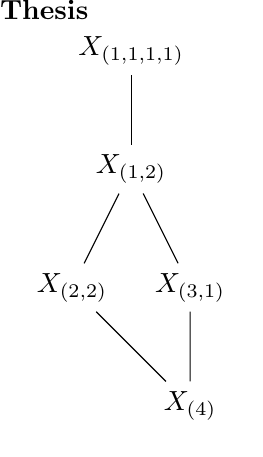
\begin{tikzpicture}
  \node {$X_{(1,1,1,1)}$}
  child {node {$X_{(1,2)}$}
    child {node[name=A] {$X_{(2,2)}$}}
    child {node {$X_{(3,1)}$}
      child {node[name=B] {$X_{(4)}$}}}};
  \draw (A) edge (B);
\end{tikzpicture}

First, note that \[X_{(2,2)}\cong\{(x,y)\in E^2:2x+2y=0\}=\{(x,y)\in E^2:x+y\text{ is 2-torsion}\}\]
so $X_{(2,2)}$ is a disjoint union of four curves each corresponding to a 2-torsion point $t_i$:
\[
C_i=\text{image}(f_i:E\hookrightarrow(\P^3)^*),\ f_i(x)=H\text{ where }H\cap E=2x+2(t_i-x)
\]
Note that $f_i$ is 2-to-1 ($x$ and $t_i-x$ are in the same fiber), so $C_i\cong E/S_2\cong\P^1$.

See ``Documents/four\_curves\_linear.m2'' for the computation in M2 to compute $X_{(2,2)}$; it turns out that each $C_i$ is a plane conic. By counting points of
intersection of the images of $C_i$ under $\pi:(\P^3)^*\dashrightarrow\P^2$, we find that
\[
N_{(4),(2,2),(2,2)}=3
\]
as expected from the Hurwitz calculation. By changing $\pi$ (and therefore $H_0$), we can also find
\[
N_{(3,1),(2,2),(2,2)}=N_{(2,2),(2,2),(2,2)}=6,\]\[ N_{(2,1,1),(2,2),(2,2)}=12,\ N_{(1,1,1,1),(2,2),(2,2)}=24
\]

Next we consider $X_{(3,1)}$ (calculated in ``osculating.m2''). There is a map $g:E\to(\P^3)^*$ sending $q\mapsto H$ where $H$ is the {\it osculating plane} to $E$ at $q$, i.e.\ $H$ intersects $E$ at
$q$ with multiplicity at least 3. This $H$ can be defined as the limit of planes containing $q,r,s\in E$ as $r,s\to q$, or equivalently as the limit of planes containing
$T_qE$ and $r$ as $r\to q$. (TODO: re-work the osculating plane stuff using that it's generated by $v(0),v'(0),v''(0)$.)

Let $E=\{F=G=0\}\subset\P^3$. We know that \[T_qE=\{x:\nabla_qF\cdot x=\nabla_qG\cdot x=0\}\]
A plane containing this tangent line must be of the form \[H=\{x:(a\nabla_qF+b\nabla_qG)\cdot x=0\}\]
for some $a,b$. If $r\in H$, then
\[
a\nabla_qF\cdot r+b\nabla_qG\cdot r=0\implies [a:b]=[\nabla_qG\cdot r:-\nabla_qF\cdot r]
\]
This equation fails when $r=q$ (since $\nabla_qF\cdot q=\nabla_qG\cdot q=0$). Letting $[u:v]$ be the limit of $[\nabla_qG\cdot r:\nabla_qF\cdot r]$
as $r\to q$, we'll have
\[
H=\left\{\left(u\frac{\partial F}{\partial x}\bigg|_q-v\frac{\partial G}{\partial x}\bigg|_q\right)x+
\left(u\frac{\partial F}{\partial y}\bigg|_q-v\frac{\partial G}{\partial y}\bigg|_q\right)y+
\left(u\frac{\partial F}{\partial z}\bigg|_q-v\frac{\partial G}{\partial z}\bigg|_q\right)z+
\left(u\frac{\partial F}{\partial w}\bigg|_q-v\frac{\partial G}{\partial w}\bigg|_q\right)w=0\right\}
\]
It remains to find $u$ and $v$. Suppose we have a (non-algebraic) parametrization of $E$ labeled $v(t)$, with $v(0)=q$. Using L'Hopital, our goal
is to find
\[
\lim_{t\to 0}[\nabla_qG\cdot v(t):\nabla_qF\cdot v(t)]=\lim_{t\to 0}[\nabla_qG\cdot v'(t):\nabla_qF\cdot v'(t)]=\lim_{t\to 0}[\nabla_qG\cdot v''(t):\nabla_qF\cdot v''(t)]=[\nabla_qG\cdot v''(0):\nabla_qF\cdot v''(0)]
\]


We know
$F(v(t))=0$ and $G(v(t))=0$ so
\[
\nabla _{v(t)}F\cdot v'(t)=\nabla _{v(t)}G\cdot v'(t)=0
\]
Taking derivatives again,
\[
\nabla_{v(t)}F\cdot v''(t)+v'(t)\cdot\left(\frac{\partial^2F}{\partial t_i\partial t_j}\right)\cdot v'(t)=\nabla_{v(t)}G\cdot v''(t)+v'(t)\cdot\left(\frac{\partial^2G}{\partial t_i\partial t_j}\right)\cdot v'(t)=0
\]
It remains to compute $v'(0)\cdot H\cdot v'(0)$ where $H$ is the Hessian of $F$ or $G$.
We know that $v'(0)$ is in the kernel of $\nabla_qF$ and $\nabla_qG$ and any generic element of both kernels will work, so we choose an element of the kernel of
\[
\begin{bmatrix}
  \frac{\partial F}{\partial x}\big|_q & \frac{\partial F}{\partial y}\big|_q & \frac{\partial F}{\partial z}\big|_q & \frac{\partial F}{\partial w}\big|_q \\
  \frac{\partial G}{\partial x}\big|_q & \frac{\partial G}{\partial y}\big|_q & \frac{\partial G}{\partial z}\big|_q & \frac{\partial G}{\partial w}\big|_q \\
  1 & 0 & 0 & 0 \\
  \end{bmatrix}
\]
It turns out $[D_1,-D_2,D_3,-D_4]$ works where $D_i$ is the determinant of the matrix produced by deleting the $i^{\text{th}}$ column, which can be shown by duplicating rows and taking determinants
(which will be 0).

After doing this it turns out that $X_{(1,3)}$ is a degree 12 curve, with singularities (cusps? TODO) at the planes $H$ with $H\cap E=4q$ for some $q$ (corresponding to the 4-torsion points). There are $4^2=16$ of these singularities.

To compute $N_{(4),(3,1),(3,1)}$, we take the image $Y_{(1,3)}$ under projection from $H_0$. It turns out that $Y_{(1,3)}$ is a degree 10
curve with cusps at the images of 4-torsion points (except for the image of $H_0$, which is a smooth point) and $20$ nodes, so
\[
N_{(4),(3,1),(3,1)}=\frac{20}{2}=10
\]
TODO: calculate $N_{(1,1,1,1),(3,1),(3,1)}$ using genus-degree formula; explain why this doesn't work for higher degree

\subsection{Admissible covers}

We may also calculate $W_{\mu,\sigma_2,\dots,\sigma_n}$ as follows when $|\mu|\geq 2$:

Consider a special genus $1$ stable curve $C$ with $|\mu|$ marked points, obtained by taking
a generic genus $1$ curve with $|\mu|-1$ marked points and gluing a genus $0$ tail with $3$ marked points.
In other words, we consider a generic point $C$ in the image of the gluing map
\[
\overline{\mathcal M}_{1,|\mu|-1}\times\overline{\mathcal M}_{0,3}\to \overline{\mathcal M}_{1,|\mu|}
\]
We will compute the number of admissible covers $\pi:C\to C'$ where $C'$ is a genus $0$ prestable curve and
$\pi$ has the ramification needed for $W_{\mu,\sigma_2,\dots,\sigma_n}$.

TODO: Explain process for calculating $N$ and/or $W$ via admissible covers
diagrams; prove that both methods (labeled and unlabeled) work

Show how reduction to $g=0$ works

\section{All twos case}

In this section we study the invariants $N_{\mu,(2^k),(2^k)}$ defined for $d=2k$ even.
We will ultimately prove that
\[
N_{\mu,(2^k),(2^k)}=3\cdot 2^{\ell(\mu)-1},
\]
along the way demonstrating techniques to compute our invariants, which will prove the result in special instances.

First, we will translate the calculation of $N_{\mu,(2^k),(2^k)}$ into a problem of intersection theory
in projective space, which we will solve in the special case where $\mu=(1^d)$.
We will then calculate the opposite extreme case, where $\mu=(d)$, first by use of Hurwitz theory and
secondly by a genus reduction technique. Finally, we will establish the result in full generality using
our most powerful technique: establishing a recursion between these invariants by use of
our admissible covers technique, which yields the full solution in combination with either of the base
cases we have computed.

\subsection{Motivation}

The Gromov-Witten invariants of an elliptic curve are well understood. However, a natural generalization
remains open: let $C$ be the quotient of an elliptic curve under the action $x\mapsto -x$.
This action has $4$ fixed points (the two-torsion points in the group law), and so as an orbifold
$C$ can be identified as $\P^1$ with $4$ points of stabilizer $\Z/2$, and is known as the
{\it pillowcase orbifold}. Maps $E\to C$ correspond to maps $E\to\P^1$ with ``even'' ramification over
the $4$ special points, and so $N_{\mu,(2^k),(2^k)}$ can be interpreted as a relative Gromov-Witten
invariant of the pillowcase $C$, fitting into a larger picture of classes $\langle \mu\rangle_d^{C}\in H^{g-1}(\overline{\mathcal M}_{g,\ell(\mu)})$.

\subsection{Geometric interpretation}

The problem can be restated in geometric terms as follows: let $E\subset \P^{d-1}$ be a general genus $1$ curve,
and let $H_0$ be a general hyperplane such that $H_0\cap E$ has type $\mu$. Then letting \[X_{(2^k)}=\{H\in(\P^{d-1})^*:H\cap E\text{ is of type }(2^k)\}\]
and $\pi:(\P^{d-1})^*\dashrightarrow \P^{d-2}$ be projection away from $H_0$, we want the number of fibers of $\pi$
containing multiple points of $X_{(2^k)}$.

For any $H\in X_{(2^k)}$, we know $H\cap E=2p_1+\dots+2p_k$ for some points $p_1,\dots,p_k\in E$. Then in the group law, we have
\[
2p_1+\dots+2p_k=0\implies p_1+\dots+p_k\in\{t_1,t_2,t_3,t_4\}
\]
where the $t_i$ are the $2$-torsion points of $E$. This means we have a map $X_{(2^k)}\to\{t_1,t_2,t_3,t_4\}$ sending $H\mapsto p_1+\dots+p_k$, and since the target is discrete, $X_{(2^k)}$ can be divided into four connected components:
\[
X_{(2^k)}=X_{(2^k)}^{(1)}\cup X_{(2^k)}^{(2)}\cup X_{(2^k)}^{(3)}\cup X_{(2^k)}^{(4)}
\]
Each component is (abstractly? TODO) isomorphic to $E^{k-1}/\sim\cong \P^{k-1}$,
and our goal is to count the size of $\pi(X_{(2^k)}^{(i)})\cap \pi(X_{(2^k)}^{(j)})$
for $i\neq j$.

It will be necessary to compute the degree of $X_{(2^k)}$, so we begin with a more general calculation of the degree of $X_{\mu}$:

\begin{lem}
  If $\mu=(\mu_1,\dots,\mu_n)$ with $|\mu|=d$, then
  \[
  \text{deg}(X_{\mu})=\frac{\mu_1\cdots\mu_n\cdot d(n-1)!}{|\text{Aut}(\mu)|}
  \]
\end{lem}

\begin{proof}
  We use Proposition 5.1, p 358 of ``Geometry of Algebraic Curves'' by Arbarello, Cornalba, Griffiths and Harris. Considering the map
  $\phi:E^n\to\text{Sym}^dE$ sending $(x_1,\dots,x_n)\mapsto \sum_{i=1}^n\mu_ix_i$,
  the degree we want is the restriction of $x^{n-1}[\text{im}(\phi)]$ to
  the divisor $(\P^{d-1})^*\subset\text{Sym}^dE$ consisting of effective divisors
  equivalent to our given divisor. We know that $\theta$ vanishes when
  restricted to our $(\P^{d-1})^*$, so we only need consider the case $\alpha=\beta=0$ in the Proposition and
  \begin{align*}
    \phi_*[E^n]x^{n-1}\bigg|_{(\P^{d-1})^*}&=[(1+\mu_1t_1+\dots+\mu_nt_n)^{n-1}(1+\mu_1^2t_1+\dots+\mu_n^2t_n)]_{t_1\cdots t_n}\\
    &=\sum_{i=1}^n(n-1)!(\mu_1\cdots\hat{\mu_i}\cdots \mu_n)\cdot\mu_i^2\\
    &=(n-1)!\mu_1\cdots\mu_n\cdot (\mu_1+\dots+\mu_n)
  \end{align*}

  
  The map $\phi$ is $|\Aut(\mu)|$-to-1, and so we end up with our result.
  \end{proof}
In particular,
\[
\text{deg}(X_{(2^k)})=\frac{(k-1)!2^k(2k)}{k!}=2^{k+1}\implies \text{deg}(X_{(2^k)}^{(i)})=2^{k-1}.
\]
Let $\mu=(1^{d})$. Then the intersection is the sum of product of degrees of $X_{(2^k)}^{(i)}$ and $X_{(2^k)}^{(j)}$ for $i\neq j$, i.e.
\[
\binom 42\cdot 2^{k-1}\cdot 2^{k-1}=6\cdot 2^{d-2}=3\cdot 2^{d-1}
\]
in agreement with our main claim.


\subsection{$\mu=(d)$}

Having proved the result geometrically for $\mu=(1,\dots,1)$, we now tackle the other extreme case, where $\mu=(d)$. We will show that $N_{(d),(2^k),(2^k)}=3$
using two methods: first, by categorizing all such maps explicitly using Hurwitz theory and counting them, and second by performing a genus reduction.

\subsubsection{Combinatorial solution}


\includegraphics[scale=0.2]{diagram.jpg}

\includegraphics[angle=90,scale=0.15]{diagram2.jpg}

\begin{claim}
  Let $f:E\to\P^1$ be of degree $d=2k$ such that $f(p)=0$ with full ramification,
  and $f$ has ramification profiles $(2^k)$ over $1$ and $\infty$. Then $f$ factors as
  $E\to\P^1\to\P^1$ where the first map is degree $2$ and the second is degree $k$.
\end{claim}
\begin{proof}
  The pictures above illustrate how such maps should factor. We prove the claim by fixing branch points $0,1,\infty,w$ in $\P^1$, counting the (orbifold) number of factored
  maps over these branch points as well as the maps in the last picture, and show that these are equal.

  The latter count is given by
  \[
  H((d),(2^k),(2^k),(2,1,\dots,1))
  \]
  which is $k/2$ by the Appendix. For the former count, we
  first consider maps $\P^1\to\P^1$  (with $0,1,\infty,w$ fixed)
  described in the picture (depending on the parity of $k$). These
  are counted by
  $H((k),(2^{(k-1)/2},1),(2^{(k-1)/2},1))$ if $k$ is odd or
  $H((k),(2^{k/2-1},1,1),(2^{k/2}))$ if $k$ is even, both of which are $1$
  by results of the Appendix. The count for the upstairs map $E\to\P^1$ is
  $H((2),(2),(2),(2))=\frac 12$ multiplied by the number of options for point $d$
  (which is $k$). Thus, the orbifold number of factored maps lying over $0,1,\infty,w$ is $1\cdot \frac 12\cdot k$, proving the claim.
  
\end{proof}

Now given this result, we can compute $N_{(d),(2^k),(2^k)}$ by counting
the number of factored maps described in the picture for a fixed $(E,p)$.
The map $(E,p)\to(\P^1,a)$ is the elliptic map to $\P^1$ and therefore unique up
to automorphisms of $\P^1$ fixing $a$; there are $3$ choices for the point
$d$, and after this the map is uniquely determined up to automorphisms of
$\P^1$ (by the Hurwitz counts above). Therefore,
\[
N_{(d),(2^k),(2^k)}=3.
\]

\subsubsection{Genus reduction}

Consider a genus $0$ curve with a self-node, along
with a marked point $p$. There are two kinds of
admissible covers from this curve to $\P^1$
with ramification $(d),(2^k),(2^k),(2,1,\dots,1)$:


            \begin{tikzpicture}[thick,amat/.style={matrix of nodes,nodes in empty cells,
  row sep=3.2em,rounded corners,
  nodes={draw,solid,circle,minimum size=1.5cm}},
  dmat/.style={matrix of nodes,nodes in empty cells,row sep=3.2em,nodes={minimum size=1.5cm},draw=myred},
  fsnode/.style={fill=myblue},
  ssnode/.style={fill=mygreen}]

  \matrix[amat,nodes=fsnode] (mat1) {$0$\\};

    \matrix[dmat,left=1cm of mat1] (degrees1) {$d$\\};


 \matrix[amat,right=4cm of mat1,nodes=ssnode] (mat2) {$0$\\};

 \matrix[dmat,right=1cm of mat2] (degrees2) {$d$\\};

 \draw  (mat1-1-1) edge["$a$",bend left] (mat2-1-1)
 (mat1-1-1) edge["$b$"] (mat2-1-1);

  % draw legs for left side
 \draw (mat1-1-1) -- +(95:1) node[anchor=south] {$p$}
 (mat1-1-1) -- +(245:1) node[anchor=north] {$(2,1^{d-2})$};

 % draw legs for right side
 \draw  (mat2-1-1) -- +(30:1) node[anchor=west] {$(2^k)$}
 (mat2-1-1) -- +(330:1) node[anchor=west] {$(2^k)$};

            \end{tikzpicture}
            
            \begin{tikzpicture}[thick,amat/.style={matrix of nodes,nodes in empty cells,
  row sep=3.2em,rounded corners,
  nodes={draw,solid,circle,minimum size=1.5cm}},
  dmat/.style={matrix of nodes,nodes in empty cells,row sep=3.2em,nodes={minimum size=1.5cm},draw=myred},
  fsnode/.style={fill=myblue},
  ssnode/.style={fill=mygreen}]

  \matrix[amat,nodes=fsnode] (mat1) {$0$\\};

    \matrix[dmat,left=1cm of mat1] (degrees1) {$d$\\};


 \matrix[amat,right=4cm of mat1,nodes=ssnode] (mat2) {$0$\\
      $0$\\
      $\vdots$\\
  $0$\\};

 \matrix[dmat,right=1cm of mat2] (degrees2) {$2$\\
   $2$ \\
    \vdots \\
    $2$\\};

 \draw  (mat1-1-1) edge["$1$",bend left] (mat2-1-1)
 (mat1-1-1) edge["$1$"] (mat2-1-1)
 (mat1-1-1) edge["$2$"] (mat2-2-1)
 (mat1-1-1) edge["$2$"] (mat2-4-1);

  % draw legs for left side
 \draw (mat1-1-1) -- +(95:1) node[anchor=south] {$p$}
 (mat1-1-1) -- +(245:1) node[anchor=north] {$(2^k)$};

 % draw legs for right side
 \draw  (mat2-1-1) -- +(30:1) node[anchor=west] {$2$}
 (mat2-1-1) -- +(330:1) node[anchor=west] {$2$}
 (mat2-2-1) -- +(330:1) node[anchor=west] {$2$}
 (mat2-4-1) -- +(330:1) node[anchor=west] {$2$};

          \end{tikzpicture}

            TODO: perform counts for these diagrams

\section{$S_{\a,\b}$}

\subsection{Definitions and basic results}

Let
\[
S_{\mathfrak a,\mathfrak b}(\mu)=N_{\mu,(2,1,\dots)^{a_2},(2,1,\dots)^{b_2},(3,1,\dots)^{a_3},(3,1,\dots)^{b_3},\dots}^{\{2^{b_2}3^{b_3}\dots\}}
\]
Here $a_2,a_3,\dots$ describe unmarked ramification and $b_2,b_3,\dots$ describe marked ramification. For
simplicity, assume that all ramification is included and define $S_{\mathfrak a,\mathfrak b}(\mu)= 0$ if $\mu_i\leq 0$ for any $i$.

\begin{lem}
  If $S_{\mathfrak a,\mathfrak b}(\mu)$ is well-defined, $|\mathfrak a|=|\mu|+2$.
\end{lem}
\begin{proof}
  Let $\mathcal X$ be the moduli space of maps from a genus $1$ curve to $\mathbb P^1$, with ramification as required for $S_{\mathfrak a,\mathfrak b}(\mu)$, and with all relevant points of the genus $1$ curve marked
  (corresponding to $\mathfrak a$, $\mathfrak b$, and $\mu$). There is a map $\mathcal X\to\overline{\mathcal M}_{1,|\mathfrak b|+|\mu|}$ remembering the genus $1$ curve and the fixed points, which is finite by assumption, so $\dim(\mathcal X)=|\mathfrak b|+|\mu|$. There is also a map $\mathcal X\to\overline{\mathcal M}_{0,|\mathfrak a|+|\mathfrak b|+1}$ remembering the branch points of the target, which is finite by Hurwitz's theorem, and so
  \[
  |\mathfrak b|+|\mu|=\dim(\overline{\mathcal M}_{0,|\mathfrak a|+|\mathfrak b|+1})=|\mathfrak a|+|\mathfrak b|-2
  \]
  yielding the result.
\end{proof}

\subsection{Reduction of $\b$}
\begin{claim}[Claim 1]
  For $n>0$, if $b_y>0$, then
  \begin{align*}
    S_{\mathfrak a,\mathfrak b+\{y\}}(\mu, n) &=S_{\mathfrak a,\mathfrak b}(\mu, n-y+1) +\sum_{z\in\mathfrak a}\min(z-1,y-1,n,y+z-n-2)S_{\mathfrak a-\{z\},\mathfrak b+\{y+z-n-2\}}(\mu)
  \end{align*}
\end{claim}

\begin{proof}
  We consider diagrams which stabilize to a genus $1$ curve containing $x_1,\dots,x_k$ and all but one
  of the other fixed points, attached to a genus $0$ tail containing $q$ (with ramification $n$) and $p$
  (with ramification $y$).

  First, note that the total number of branch points for any such map should be $|\mathfrak a|+|\mathfrak b|+1$.
  Restricting to the genus $1$ component, the moduli space of maps for that component has a finite map to $\overline{\mathcal M}_{1,|\mathfrak b|+k}$ and therefore has dimension $|\mathfrak b|+k$, so the number of branch points is $|\mathfrak b|+k+3$. One
  of these branch points is the node of the target genus $0$, so discounting this there are $|\mathfrak b|+k+2$ proper branch points.
  Therefore, the number of branch points outside the genus $1$ component is
  \[
  (|\mathfrak a|+|\mathfrak b|+1)-(|\mathfrak b|+k+2)=|\mathfrak a|-k-1=|\mathfrak a|-|(\mu,n)|=2
  \]
  by the lemma.
  
  A diagram with $x_1,\dots,x_k$ on the right side looks like:

\begin{tikzpicture}[thick,amat/.style={matrix of nodes,nodes in empty cells,
  row sep=3.2em,rounded corners,
  nodes={draw,solid,circle,minimum size=1.5cm}},
  dmat/.style={matrix of nodes,nodes in empty cells,row sep=3.2em,nodes={minimum size=1.5cm},draw=myred},
  fsnode/.style={fill=myblue},
  ssnode/.style={fill=mygreen}]

  \matrix[amat,nodes=fsnode] (mat1) {$1$\\
    $0$\\
    \vdots \\
  $0$\\};

  \matrix[dmat,left=2cm of mat1] (degrees1) {$d-\sum c_i$\\
    $c_1$\\
    \vdots \\
  $c_r$\\};

 \matrix[amat,right=7cm of mat1,nodes=ssnode] (mat2) {$0$\\
   \vdots\\
   $0$ \\
   $0$\\};
 \matrix[dmat,right=1.5cm of mat2] (degrees2) {$\mu_1$\\
   \vdots\\
   $\mu_k$ \\
 $n$\\};

 \draw  (mat1-1-1) edge["$\mu_1$"] (mat2-1-1)
 (mat1-1-1) edge["$\mu_k$"] (mat2-3-1)
 (mat1-1-1) edge["$n-\sum c_i$"] (mat2-4-1)
 (mat1-2-1) edge["$c_1$"] (mat2-4-1)
 (mat1-4-1) edge["$c_r$"] (mat2-4-1);

  % draw legs for left side
 \draw (mat1-1-1) -- +(95:1) node[anchor=south] {fixed points};

 % draw legs for right side
 \draw  (mat2-1-1) -- +(30:1) node[anchor=west] {$x_1$}
 (mat2-3-1) -- +(30:1) node[anchor=west] {$x_k$}
 (mat2-4-1) -- +(30:1) node[anchor=west] {$q$};

\end{tikzpicture}

There are two branch points outside the genus $1$ component, which must be the images of
$x_1,\dots,x_k,q$ and of $p$. This means there is no extra ramification on any genus $0$ component, which is why each top right bubble
connects only to the genus $1$ component. The bottom right bubble must have some ramification beyond what is pictured here, which is necessarily
$p$. So our diagram looks like:

  \begin{tikzpicture}[thick,amat/.style={matrix of nodes,nodes in empty cells,
  row sep=3.2em,rounded corners,
  nodes={draw,solid,circle,minimum size=1.5cm}},
  dmat/.style={matrix of nodes,nodes in empty cells,row sep=3.2em,nodes={minimum size=1.5cm},draw=myred},
  fsnode/.style={fill=myblue},
  ssnode/.style={fill=mygreen}]

  \matrix[amat,nodes=fsnode] (mat1) {$1$\\
    $0$\\
    \vdots \\
  $0$\\};

  \matrix[dmat,left=2cm of mat1] (degrees1) {$d-r$\\
    $1$\\
    \vdots \\
  $1$\\};

 \matrix[amat,right=7cm of mat1,nodes=ssnode] (mat2) {$0$\\
   \vdots\\
   $0$ \\
   $0$\\};
 \matrix[dmat,right=1.5cm of mat2] (degrees2) {$\mu_1$\\
   \vdots\\
   $\mu_k$ \\
 $n$\\};

 \draw  (mat1-1-1) edge["$\mu_1$"] (mat2-1-1)
 (mat1-1-1) edge["$\mu_k$"] (mat2-3-1)
 (mat1-1-1) edge["$n-r$"] (mat2-4-1)
 (mat1-2-1) edge["$1$"] (mat2-4-1)
 (mat1-4-1) edge["$1$"] (mat2-4-1);

  % draw legs for left side
 \draw (mat1-1-1) -- +(95:1) node[anchor=south] {fixed points};

 % draw legs for right side
 \draw  (mat2-1-1) -- +(30:1) node[anchor=west] {$x_1$}
 (mat2-3-1) -- +(30:1) node[anchor=west] {$x_k$}
 (mat2-4-1) -- +(30:1) node[anchor=west] {$q$}
 (mat2-4-1) -- +(330:1) node[anchor=west] {$p$};

  \end{tikzpicture}

  As there is no extra ramification outside the genus $1$ component,
  the dimension reduction of $r$ should match the codimension reduction
  corresponding to the removal of $p$, which is $y-1$. So $r=y-1$ and we
  have the first term in the claim, since $H((n),(y,1,\dots),(n-y+1,1,\dots))=1$.

  Now consider the case where $x_1,\dots,x_k,q$ are on the left side. In this
  case, the branch points not coming from the genus $1$ component will be
  the image of $p$ and the image of another point $p'$ (with ramification index $z\in\mathfrak a$). Consider the possibility that
  $x_1,\dots,x_k$ are not all on the genus $1$ component:

  \begin{tikzpicture}[thick,amat/.style={matrix of nodes,nodes in empty cells,
  row sep=3.2em,rounded corners,
  nodes={draw,solid,circle,minimum size=1cm}},
  dmat/.style={matrix of nodes,nodes in empty cells,row sep=3.2em,nodes={minimum size=1cm},draw=myred},
  fsnode/.style={fill=myblue},
  ssnode/.style={fill=mygreen}]

    \matrix[amat,nodes=fsnode] (mat1) {$0$\\
      $1$\\};

    \matrix[amat,right=2cm of mat1,nodes=ssnode] (mat2) {$0$\\};

      \matrix[dmat,left=1cm of mat1] (degrees1) {$\mu_1$\\
    $d-n-\mu_1$\\};

            \matrix[dmat,right=0.5cm of mat2] (degrees2) {$e$\\};
  
 \draw  (mat1-1-1) edge["$\mu_1$"] (mat2-1-1)
 (mat1-2-1) edge["$e-\mu_1$"] (mat2-1-1);

  % draw legs for left side
 \draw (mat1-1-1) -- +(120:1) node[anchor=south] {$x_1$}
 (mat1-2-1) -- +(120:1) node[anchor=south] {$x_2,\dots,x_k$};

   % draw legs for right side
 \draw (mat2-1-1) -- +(100:1) node[anchor=south] {$e$ ramif};


  \end{tikzpicture}

  This would require the genus $0$ on the right side to have multiple branch points contributing
  $e$ ramification,
  but $p$ cannot live on this component (because of the stabilization condition), a contradiction.
  Therefore, $x_1,\dots,x_k$ all live on the genus $1$ component.

  The points $p$ and $p'$ cannot lie on separate components, because the following diagram cannot be completed:

        \begin{tikzpicture}[thick,amat/.style={matrix of nodes,nodes in empty cells,
  row sep=3.2em,rounded corners,
  nodes={draw,solid,circle,minimum size=1.5cm}},
  dmat/.style={matrix of nodes,nodes in empty cells,row sep=3.2em,nodes={minimum size=1.5cm},draw=myred},
  fsnode/.style={fill=myblue},
  ssnode/.style={fill=mygreen}]

  \matrix[amat,nodes=fsnode] (mat1) {$1$\\
    $0$\\};

  \matrix[dmat,left=2cm of mat1] (degrees1) {$d-n$\\
    $n$\\};

 \matrix[amat,right=3cm of mat1,nodes=ssnode] (mat2) {$0$\\
   $0$\\};
 \matrix[dmat,right=1.5cm of mat2] (degrees2) {$z$\\
   $y$\\};

 \draw  (mat1-2-1) edge["$y$"] (mat2-2-1);

  % draw legs for left side
 \draw (mat1-1-1) -- +(115:1) node[anchor=south] {fixed points}
 (mat1-1-1) -- +(260:1) node[anchor=north] {$x_1,\dots,x_k$}
 (mat1-2-1) -- +(260:1) node[anchor=east] {$q$};

   % draw legs for right side
 \draw (mat2-1-1) -- +(75:1) node[anchor=south] {$p'$}
 (mat2-2-1) -- +(265:1) node[anchor=north] {$p$};


 \end{tikzpicture}

  Therefore $p$ and $p'$ lie on the same genus $0$ component, all other genus $0$ components on the right side have degree $1$,
  and we end up with:
  
        \begin{tikzpicture}[thick,amat/.style={matrix of nodes,nodes in empty cells,
  row sep=3.2em,rounded corners,
  nodes={draw,solid,circle,minimum size=1.5cm}},
  dmat/.style={matrix of nodes,nodes in empty cells,row sep=3.2em,nodes={minimum size=1.5cm},draw=myred},
  fsnode/.style={fill=myblue},
  ssnode/.style={fill=mygreen}]

  \matrix[amat,nodes=fsnode] (mat1) {$1$\\
    $0$\\};

  \matrix[dmat,left=2cm of mat1] (degrees1) {$d-n$\\
    $n$\\};

 \matrix[amat,right=3cm of mat1,nodes=ssnode] (mat2) {$0$\\
   \vdots\\
   $0$ \\
   $0$\\};
 \matrix[dmat,right=1.5cm of mat2] (degrees2) {$1$\\
   \vdots\\
   $1$ \\
   $e+n$\\};

 \draw  (mat1-1-1) edge["$1$"] (mat2-1-1)
 (mat1-1-1) edge["$1$"] (mat2-3-1)
 (mat1-1-1) edge["$e$"] (mat2-4-1)
 (mat1-2-1) edge["$n$"] (mat2-4-1);

  % draw legs for left side
 \draw (mat1-1-1) -- +(115:1) node[anchor=south] {fixed points}
 (mat1-1-1) -- +(260:1) node[anchor=north] {$x_1,\dots,x_k$}
 (mat1-2-1) -- +(140:1) node[anchor=east] {$q$};

   % draw legs for right side
 \draw (mat2-4-1) -- +(75:1) node[anchor=south] {$p$}
 (mat2-4-1) -- +(265:1) node[anchor=north] {$p'$};


        \end{tikzpicture}

        By Riemann-Hurwitz for the bottom-right component, 
        \[
        (e+n-2)+(y-1)+(z-1)=2(e+n)-2\implies y+z-2=e+n\implies e=y+z-n-2.
        \]
        By our calculation of $H((y+z-n-2,n),(z,1,\dots),(y,1,\dots))$ (and noting that
        we should multiply by $2$ if $y+z-n-2=n$, since the corresponding edges should be
        distinguished), we end up with the term in the claim.
        
\end{proof}

\subsection{Reduction of $\a$}
\begin{claim}[Claim 2]
  For $n>0$,
  \begin{align*}
    S_{\mathfrak a,\mathfrak b}(\mu, n, m) &= \sum_{z\in\mathfrak a,\ z\leq n+m}\min(n,m,z-1,n+m-z+1)S_{\a-\{z\},\b}(\mu,n+m-z+2) \\
    &+\sum_{z_1,z_2\in\a-\{2\}}\hat H((z_1+z_2-n-m-3,n,m),(z_1,1,\dots),(z_2,1,\dots))S_{\a-\{z_1,z_2\},\b+\{z_1+z_2-n-m-3\}}(\mu)
  \end{align*}
\end{claim}
Here $\hat H$ means  ``multiply by $|\Aut(n,m,z_1+z_2-n-m-3)|/|\Aut(z_1,z_2)|$''.

\begin{proof}
    We consider diagrams which stabilize to a genus $1$ curve containing $x_1,\dots,x_k$ and all 
  of the other fixed points, attached to a genus $0$ tail containing $q$ (with ramification index $n$) and $r$
  (with ramification index $m$).
  
  By reasoning as in the last claim, the number of branch points not coming from the genus $1$ component is
  \[
  (|\mathfrak a|+|\mathfrak b|+1)-(|\b|+k+3)=|\a|-|(\mu,n,m)|=2.
  \]
  If $x_1,\dots,x_k,q,r$ are on the right side, then there is one more branch point arising as the image of some $s$ (with
  ramification index $z$). Suppose $q$ and $r$ are on different components:

  \begin{tikzpicture}[thick,amat/.style={matrix of nodes,nodes in empty cells,
  row sep=3.2em,rounded corners,
  nodes={draw,solid,circle,minimum size=1.5cm}},
  dmat/.style={matrix of nodes,nodes in empty cells,row sep=3.2em,nodes={minimum size=1.5cm},draw=myred},
  fsnode/.style={fill=myblue},
  ssnode/.style={fill=mygreen}]

  \matrix[amat,nodes=fsnode] (mat1) {$1$\\
    $0$\\};

 \matrix[amat,right=7cm of mat1,nodes=ssnode] (mat2) {$0$\\
   \vdots\\
   $0$ \\
   $0$\\
 $0$\\};

 \draw  (mat1-1-1) edge["$\mu_1$"] (mat2-1-1)
 (mat1-1-1) edge["$\mu_k$"] (mat2-3-1)
 (mat1-1-1) edge["$c$"] (mat2-4-1)
 (mat1-2-1) edge["$e$"] (mat2-4-1)
 (mat1-2-1) edge["$m$"] (mat2-5-1);

  % draw legs for left side
 \draw (mat1-1-1) -- +(95:1) node[anchor=south] {fixed points};

 % draw legs for right side
 \draw  (mat2-1-1) -- +(30:1) node[anchor=west] {$x_1$}
 (mat2-3-1) -- +(30:1) node[anchor=west] {$x_k$}
 (mat2-4-1) -- +(30:1) node[anchor=west] {$q$}
 (mat2-5-1) -- +(30:1) node[anchor=west] {$r$};

  \end{tikzpicture}

  (Without loss of generality, we suppose the component containing $q$ is the one that connects to the genus $1$.)
  There is extra ramification on both the component containing $q$ and the lower left component, a contradiction. Therefore
  $q$ and $r$ lie on the same component, and our picture must look like:

    \begin{tikzpicture}[thick,amat/.style={matrix of nodes,nodes in empty cells,
  row sep=3.2em,rounded corners,
  nodes={draw,solid,circle,minimum size=1.5cm}},
  dmat/.style={matrix of nodes,nodes in empty cells,row sep=3.2em,nodes={minimum size=1.5cm},draw=myred},
  fsnode/.style={fill=myblue},
  ssnode/.style={fill=mygreen}]

  \matrix[amat,nodes=fsnode] (mat1) {$1$\\
    $0$\\
    \vdots\\
    $0$\\};

    \matrix[dmat,left=1cm of mat1] (degrees1) {$d-e$\\
    $1$\\
    \vdots \\
  $1$\\};


 \matrix[amat,right=8cm of mat1,nodes=ssnode] (mat2) {$0$\\
   \vdots\\
   $0$ \\
   $0$\\};

     \matrix[dmat,right=1cm of mat2] (degrees2) {$\mu_1$\\
    \vdots \\
    $\mu_k$\\
     $n+m$\\};

 \draw  (mat1-1-1) edge["$\mu_1$"] (mat2-1-1)
 (mat1-1-1) edge["$\mu_k$"] (mat2-3-1)
 (mat1-1-1) edge["$n+m-e$"] (mat2-4-1)
 (mat1-2-1) edge["$1$"] (mat2-4-1)
 (mat1-4-1) edge["$1$"] (mat2-4-1);

  % draw legs for left side
 \draw (mat1-1-1) -- +(95:1) node[anchor=south] {fixed points};

 % draw legs for right side
 \draw  (mat2-1-1) -- +(30:1) node[anchor=west] {$x_1$}
 (mat2-3-1) -- +(30:1) node[anchor=west] {$x_k$}
 (mat2-4-1) -- +(30:1) node[anchor=west] {$q$}
 (mat2-4-1) -- +(50:1) node[anchor=west] {$r$}
 (mat2-4-1) -- +(300:1) node[anchor=west] {$s$};

    \end{tikzpicture}

    By Riemann-Hurwitz for the lower right component,
    \[
    (n+m-e-1)+(n+m-2)+(z-1)=2(n+m)-2\implies e=z-2
    \]
    yielding the first term in the claim using our calculation of Hurwitz numbers to simplify
    $H((n,m),(z,1,\dots),(n+m-z+2,1,\dots))$.

    If $x_1,\dots,x_k,q,r$ are on the left side, then there are two branch points arising as the images of $s_1$ (with
    ramification index $z_1$) and $s_2$ (with ramification index $z_2$). By logic similar to the last proof, the
    $x_1,\dots,x_k$ all lie on the genus $1$ component.

    Consider the possibility that $q$ and $r$ lie on the same component:

      \begin{tikzpicture}[thick,amat/.style={matrix of nodes,nodes in empty cells,
  row sep=3.2em,rounded corners,
  nodes={draw,solid,circle,minimum size=1.5cm}},
  dmat/.style={matrix of nodes,nodes in empty cells,row sep=3.2em,nodes={minimum size=1.5cm},draw=myred},
  fsnode/.style={fill=myblue},
  ssnode/.style={fill=mygreen}]

  \matrix[amat,nodes=fsnode] (mat1) {$1$\\
    $0$\\};

 \matrix[amat,right=7cm of mat1,nodes=ssnode] (mat2) {$0$\\
   \vdots\\
   $0$ \\
 $0$\\};

 \draw  (mat1-1-1) edge["$1$"] (mat2-1-1)
 (mat1-1-1) edge["$1$"] (mat2-3-1)
 (mat1-1-1) edge["$c$"] (mat2-4-1)
 (mat1-2-1) edge["$n+m$"] (mat2-4-1);

  % draw legs for left side
 \draw (mat1-1-1) -- +(95:1) node[anchor=south] {fixed points}
 (mat1-1-1) -- +(270:1) node[anchor=north] {$x_1,\dots,x_k$}
 (mat1-2-1) -- +(270:1) node[anchor=north] {$q$}
 (mat1-2-1) -- +(255:1) node[anchor=north] {$r$};

      \end{tikzpicture}

      There must be at least one additional branch point from the lower left component and at least two additional branch
      points from the lower right component, a contradiction. Therefore, $q$ and $r$ lie on separate components:

          \begin{tikzpicture}[thick,amat/.style={matrix of nodes,nodes in empty cells,
  row sep=3.2em,rounded corners,
  nodes={draw,solid,circle,minimum size=1.5cm}},
  dmat/.style={matrix of nodes,nodes in empty cells,row sep=3.2em,nodes={minimum size=1.5cm},draw=myred},
  fsnode/.style={fill=myblue},
  ssnode/.style={fill=mygreen}]

  \matrix[amat,nodes=fsnode] (mat1) {$1$\\
    $0$\\
    $0$\\};

    \matrix[dmat,left=1cm of mat1] (degrees1) {$d-n-m$\\
    $n$\\
  $m$\\};


 \matrix[amat,right=4cm of mat1,nodes=ssnode] (mat2) {$0$\\
   \vdots\\
   $0$ \\
   $0$\\};

     \matrix[dmat,right=1cm of mat2] (degrees2) {$1$\\
    \vdots \\
    $1$\\
     $c+n+m$\\};

 \draw  (mat1-1-1) edge["$1$"] (mat2-1-1)
 (mat1-1-1) edge["$1$"] (mat2-3-1)
 (mat1-1-1) edge["$c$"] (mat2-4-1)
 (mat1-2-1) edge["$n$"] (mat2-4-1)
 (mat1-3-1) edge["$m$"] (mat2-4-1);

  % draw legs for left side
 \draw (mat1-1-1) -- +(95:1) node[anchor=south] {fixed points}
 (mat1-1-1) -- +(245:1) node[anchor=north] {$x_1,\dots,x_k$}
 (mat1-2-1) -- +(245:1) node[anchor=north] {$q$}
 (mat1-3-1) -- +(245:1) node[anchor=north] {$r$};

 % draw legs for right side
 \draw  (mat2-4-1) -- +(30:1) node[anchor=west] {$s_1$}
 (mat2-4-1) -- +(300:1) node[anchor=west] {$s_2$};

          \end{tikzpicture}
          
          By Riemann-Hurwitz for the lower-right component,
          \[
          (c+n+m-3)+(z_1-1)+(z_2-1)=2(c+n+m)-2\implies c=z_1+z_2-n-m-3
          \]
          yielding the second term of the claim. The additional factors arise because
          the edges from the bottom right component should be distinguished, while $s_1$ and
          $s_2$ should not be distinguished.
\end{proof}

Claim 1 allows us to reduce to the case where $\b=\emptyset$, and Claim 2 allows us to reduce to
the case where $\mu=(d)$. It remains to calculate $S_{\{a_1,a_2,a_3\},\emptyset}(d)$ as a base case:

\begin{claim}
  When $\a=\{a_1,a_2,a_3\}$, $S_{\a,\emptyset}(d)$ is given by
  \[
  \sum_{i=1}^3\sum_{e+f=d-a_i+2}\frac{2(a_j+a_k+2) H((d),(a_1,1,\dots),(e,f,1,\dots)) H((e,f),(a_j,1,\dots),(a_k,1,\dots)) |\Aut(e,f,1^{d-e-f})|}{(a_i-2)!|\Aut(a_1,a_2,a_3)|}
  \]
  where $\{1,2,3\}=\{i,j,k\}$.
\end{claim}
\begin{proof}
  We will want to calculate $W_{(d),(a_1,1,\dots),(a_2,1,\dots),(a_3,1,\dots),(2,1,\dots)^{k}}$ (where $k=d+4-a_1-a_2-a_3$ by Riemann-Hurwitz) and then divide by \[(d-a_1)!(d-a_2)!(d-a_3)!((d-1)!)^kk!|\Aut(a_1,a_2,a_3)|\]
  The pictures to consider look like:

            \begin{tikzpicture}[thick,amat/.style={matrix of nodes,nodes in empty cells,
  row sep=3.2em,rounded corners,
  nodes={draw,solid,circle,minimum size=1.5cm}},
  dmat/.style={matrix of nodes,nodes in empty cells,row sep=3.2em,nodes={minimum size=1.5cm},draw=myred},
  fsnode/.style={fill=myblue},
  ssnode/.style={fill=mygreen}]

  \matrix[amat,nodes=fsnode] (mat1) {$0$\\};

    \matrix[dmat,left=1cm of mat1] (degrees1) {$d$\\};


 \matrix[amat,right=4cm of mat1,nodes=ssnode] (mat2) {$0$\\
      $0$\\
      $\vdots$\\
  $0$\\};

 \matrix[dmat,right=1cm of mat2] (degrees2) {$e+f$\\
   $1$
    \vdots \\
    $1$\\};

 \draw  (mat1-1-1) edge["$e$",bend left] (mat2-1-1)
 (mat1-1-1) edge["$f$"] (mat2-1-1)
 (mat1-1-1) edge["$1$"] (mat2-2-1)
 (mat1-1-1) edge["$1$"] (mat2-4-1);

  % draw legs for left side
 \draw (mat1-1-1) -- +(95:1) node[anchor=south] {$p$}
 (mat1-1-1) -- +(245:1) node[anchor=north] {$a_1$};

 % draw legs for right side
 \draw  (mat2-1-1) -- +(30:1) node[anchor=west] {$a_2$}
 (mat2-1-1) -- +(330:1) node[anchor=west] {$a_3$};

          \end{tikzpicture}

\end{proof}

\subsection{Applying recursions}

TODO: proof that Claims 1 and 2 suffice to calculate all
$S_{\a,\b}$ from base cases

We will now use the recursions to study families
\[T_n(\mu)=S_{\{n^k,2^{\ell}\},\emptyset}(\mu)\]
for fixed $n$, where $k$ is as large as possible
and then $\ell$ is determined by Riemann-Hurwitz. As a first
case, we have
\[
T_3(\mu)=S_{\{(3^{d-2}),(2^{\ell})\},\emptyset}(\mu)
\]

We find that:
\[
T_3(\mu,a,1)=T_3(\mu,a+1)+T_3(\mu,a)\text{ for $a>1$}
\]
\[
T_3(\mu,a,2)=T_3(\mu,a+2)+2T_3(\mu,a+1)\text{ for $a\geq 2$}
\]
\[
T_3(\mu,3,3)=T_3(\mu,6)+2T_3(\mu,5)
\]
and $T_3(\mu,a,b)=0$ if $a+b>6$ (for dimension reasons; TODO how does this fit with the last claim?).

\begin{claim}
  For $d\geq 3$,
  \[
  T_3(1^d)=\frac{d(d-1)(2(d-1)^2+1)}{6}
  \]
\end{claim}


TODO: Generating functions

Future questions: what does $T_n(1,\dots,1)$ look like asymptotically in $k$?

What about higher genus?

\section{Appendix 1: Hurwitz Counts}

\begin{lem}
  In the symmetric group $S_d$, let $\tau=(1\ 2)(3\ 4)\cdots (2i-1\ 2i)$
  and let $\sigma$
  be another product of $i$ disjoint transpositions, with product $X=\tau\sigma$ consisting
  of at most two disjoint cycles.

  If $\sigma$ is in the subgroup $S_{2i}\subset S_d$ (i.e. it involves only the points $1,\dots,2i$),
  then there
  exist $x_1,\dots,x_{i-1}$ such that
  \[
  \{1,\dots,2i\}=\{1,x_1,\dots,x_{i-1},\tau(1),\tau(x_1),\dots,\tau(x_{i-1})\},
  \]
  and $\sigma$ can be written as a product $\sigma=\sigma_1\cdots\sigma_i$ where:
  \begin{itemize}
  \item  $\sigma_1=(1\ x_1)$,
  \item $\sigma_j=(\tau(x_{j-2})\ x_j)$ for $1<j<i$ (here $x_0=1$),
  \item $\sigma_i=(\tau(x_{i-2})\ \tau(x_{i-1}))$.
    \end{itemize}
  
%  \[
%  \sigma=(1\ x_1)(\tau(1)\ x_2)(\tau(x_1)\ x_3)(\tau(x_2)\ x_4)(\tau(x_3)\ x_5)(\tau(x_4)\ x_6)\cdots(\tau(x_{i-3})\ x_{i-1})(\tau(x_{i-2})\ \tau(x_{i-1}))
%  \]
  
  \iffalse
  There
  \[
  \sigma=(1\ 3)(2\ 5)(4\ 7)(6\ 9)(8\ 11)\cdots (2i-4\ 2i-1)(2i-2\ 2i)
  \]
  \fi

  there
  are $\dots$ choices for $\sigma$.
\end{lem}
\begin{proof}

  We prove the claimed form of $\sigma_1,\dots,\sigma_j$ by induction on $j$. The base case $j=1$ is clear since
  there must be some transposition $(1\ x_i)$.

  Let $1<j<i$. Then by the inductive hypothesis,
  \[
  \sigma_1\cdots\sigma_{j-1}=(1\ x_1)(\tau(x_0)\ x_2)\cdots (\tau(x_{j-3})\ x_{j-1})
  \]
  If $x_{j-2}$
  
  \end{proof}

\begin{claim}
For $d=2k$ even,
\[
H((d),(2^k),(2^k),(2,1^{d-2}))=\frac k2
\]
\end{claim}

\begin{claim}
For $d=2k$ even,
\[
H((d),(2^k),(2^{k-1},1,1))=1
\]
\end{claim}

\begin{claim}
For $d=2k+1$ odd,
\[
H((d),(2^k,1),(2^{k},1))=1
\]
\end{claim}

\begin{claim}
For $2\leq a\leq d-1$,
\[
H((d),(a,1,\dots,1),(d-a+1,1,\dots,1))=1
\]
\end{claim}

\begin{claim}
  If $a+b-2=d$, $1\leq n\leq d/2$, and $2\leq a\leq d/2+1$ (equivalently $2\leq a\leq b$), then
\[
H((d-n,n),(a,1,\dots,1),(b,1,\dots,1))=\begin{cases}
\frac 12\min(a-1,n)& d=2n \\
\min(a-1,n)&\text{else}
\end{cases}
\]
\end{claim}
\begin{proof}
  We want to count choices of an $a$-cycle and a $b$-cycle which compose to produce cycle type $(d-n,n)$.
  There are $\binom da$ choices for the points of the $a$-cycle, and the
  points of the $b$-cycle are determined by the two points $x$,$y$ the cycles have in common, of which there are $\binom a2$
  choices.
  Composing these cycles yields cycle type $(n,d-n)$ where $n=n_1+n_2-1$ and
  \[
  n_1=\text{dist}_a(y,x),\quad n_2=\text{dist}_b(x,y)
  \]
  since $y$ can be traced for $n_1-1$ steps along the $a$-cycle to the predecessor of $x$, which then leads to
  the successor of $y$ in the $b$-cycle and another $n_2-1$ steps to reach $x$ again.

  If $n_1$ is fixed, there are $\frac{(a-1)!}{a-1}$ orientations of the $a$-cycle with given $\text{dist}_a(y,x)$ and similarly for the $b$-cycle,
  so our count is
  \[
  \binom da\cdot \binom a2\cdot \frac{(a-1)!}{a-1}\cdot\frac{(b-1)!}{b-1}\sum_{n_1+n_2=n+1}1
  \]
  This yields $\frac 12d!\cdot\min(a-1,n)$, and if $d\neq 2n$ then we multiply by $2$ to account for the case where $n_1+n_2-1=d-n$ instead of $n$.
  \end{proof}

\begin{claim}
  If $a+b-3=d$, $n+m+p=d$, $1\leq n\leq m\leq p$, and $3\leq a\leq \frac{d+3}{2}$ (equivalently $2\leq a\leq b$), then
\begin{align*}
  H((n,m,p),&(a,1,\dots,1),(b,1,\dots,1))\\
  &=\frac 2{|\Aut(n,m,p)|}\cdot \#\{(n_1,m_1):1\leq n_1\leq n,\ \max(1,a-p-n_1)\leq m_1\leq \min(m,a-1-n_1)\}
\end{align*}
In particular if $n=m=1$ and $d>3$, the Hurwitz number is $1$.
\end{claim}
\begin{proof}
  We want to count choices of an $a$-cycle and a $b$-cycle which compose to produce cycle type $(n,m,p)$.
  There are $\binom da$ choices for the points of the $a$-cycle, and the
  points of the $b$-cycle will be determined by the three points $x,y,z$ the cycles have in common. We have $a$ choices for
  $x$ (we will need to divide by $3$ later to account for the fact that $x,y,z$ are unordered).

  If the directionality of the $a$-cycle is $x\to y\to z\to x$ (WLOG), then the same directionality in the $b$-cycle would lead to
  a $d$-cycle, so we will require $x\to z\to y\to x$ in the $b$-cycle to end up with the desired cycle type. In this case
  we have a composed chain \[x\to\cdots\to \text{pred}_a(y)\to\text{succ}_b(y)\cdots\to x\] of length $n_1+n_2-1$ where $n_1=\text{dist}_a(x,y)$ and $n_2=\text{dist}_b(y,x)$, and similarly a composed chain
  \[
  y\to\cdots\to\text{pred}_a(z)\to\text{succ}_b(z)\to\cdots\to y
  \]
  of length $m_1+m_2-1$ where $m_1=\text{dist}_a(y,z)$ and $m_2=\text{dist}_b(z,y)$.

  Choose $n_1,n_2,m_1,m_2$ such that $n_1+n_2-1=n$ and $m_1+m_2-1=m$. Then there are $(a-1)!$ orientations of the $a$-cycle, and $y$ and $z$ are determined by $n_1$ and $m_1$. There are then $(b-3)!$ orientations of the $b$-cycle respecting the gaps $n_2$ and $m_2$. Finally, the number of choices we have in choosing $n,m$ this way out of $n,m,p$ is $\frac{3!}{|\Aut(n,m,p)|}$, so
  \begin{align*}
    H((n,m,p),(a,1,\dots,1),(b,1,\dots,1))&=\binom da\cdot a\cdot\frac 13\cdot\sum_{n_1,n_2,m_1,m_2}(a-1)!(b-3)!\cdot\frac{3!}{|\Aut(n,m,p)|} \\
    &=\frac{d!}{a!(d-a)!}\cdot\frac a3\cdot\frac{(a-1)!(d-a)!\cdot 6}{|\Aut(n,m,p)|}\#\{n_1,n_2,m_1,m_2\}
  \end{align*}
  yielding the result.
  
\end{proof}

\begin{claim}
  If $1\leq a\leq d$, $2\leq b\leq d-2$, $2\leq c\leq d-2$, and $a+b+c=d+2$, then
  \[
  H((d),(a,1,\dots),(b,c,1,\dots))=\frac{a-1}{|\Aut(b,c)|}.
  \]
  (By the first claim of this document, the Hurwitz number is $1$ if $b=1$ or $c=1$ but not both, and it is $1/d$ if $b=c=1$.)
\end{claim}
\begin{proof}
  We want to multiply an $a$-cycle by a disjoint $b$-cycle and $c$-cycle to get a $d$-cycle; the only
  requirement is that the $a$-cycle has a point $x$ contained in the $b$-cycle and a point $y$ contained in the
  $c$-cycle.
  The count is
  \[
  \binom da\cdot (a-1)!\cdot (a(a-1))\cdot \binom{d-a}{b-1}\cdot (b-1)!\cdot (c-1)!\cdot \frac 1{|\Aut(b,c)|}
  \]
  which comes out to
  \[
  d!\cdot\frac{a-1}{|\Aut(b,c)|}.
  \]
  \end{proof}


\end{document}
